\documentclass[12pt]{article}
\usepackage[utf8]{inputenc}
\usepackage{float}
\usepackage{lipsum}
\usepackage{mwe}
\usepackage{textgreek}
\usepackage[top=1in, bottom=1in, left=1in, right=1in]{geometry}
%\usepackage[margin=1in]{geometry}
\usepackage[onehalfspacing]{setspace}
%\usepackage[doublespacing]{setspace}
\usepackage{amsmath, amssymb, amsthm}
\usepackage{enumerate, enumitem}
\usepackage{fancyhdr, graphicx, proof, comment, multicol}
\usepackage[none]{hyphenat} % This command prevents hyphenation of words
\binoppenalty=\maxdimen % This command and the next prevent in-line equation breaks
\relpenalty=\maxdimen

%    Good website with common symbols
% http://www.artofproblemsolving.com/wiki/index.php/LaTeX%3ASymbols
%    How to change enumeration using enumitem package
% http://tex.stackexchange.com/questions/129951/enumerate-tag-using-the-alphabet-instead-of-numbers
%    Quick post on headers
% http://timmurphy.org/2010/08/07/headers-and-footers-in-latex-using-fancyhdr/
%    Info on alignat
% http://tex.stackexchange.com/questions/229799/align-words-next-to-the-numbering
% http://tex.stackexchange.com/questions/43102/how-to-subtract-two-equations
%    Text align left-center-right
% http://tex.stackexchange.com/questions/55472/how-to-make-text-aligned-left-center-right-in-the-same-line

\usepackage{microtype} % Modifies spacing between letters and words
\usepackage{mathpazo} % Modifies font. Optional package.
\usepackage{mdframed} % Required for boxed problems.
\usepackage{parskip} % Left justifies new paragraphs.
\linespread{1.1} 

\newcommand{\R}{\mathbb{R}}
\newcommand{\C}{\mathbb{C}}
\newcommand{\Z}{\mathbb{Z}}
\newcommand{\N}{\mathbb{N}}
\newcommand{\Q}{\mathbb{Q}}


\begin{document}
% This is the Header
% Make sure you update this information!!!!

%\noindent
\textbf{Deep Learning Lab (INF.M135)} \hfill \textbf{Marco Ferri} \\
\normalsize Università della Svizzera Italiana \hfill Due Date: 28/11/19 \\

% This is where you name your homework
\begin{center}
\textbf{Assignment 3: LSTM}
\end{center}




\section{Dataset}

For the given text-prediction problem, The Count of Monte Cristo has been chosen for creating the training dataset. Since the model is developed as a character-by-character predictor, we are interested in analyzing the source content at the character-level.

The book contains a total of about 2.65 million characters. The number of unique characters is 107: most of them are English letters and punctuation, but also numbers and Greek letters are present. Displayable characters are shown below.

\begin{verbatim}
	\n	 !	 "	 #	 $	 %	 &	 ""	 (	 )	 *	 		 -	 .	 /	 
	0	 1	 2	 3	 4	 5	 6	 7	 8	 9	 :	 ;	 ?	 @	 [	 ]	 _	 
	a	 b	 c	 d	 e	 f	 g	 h	 i	 j	 k	 l	 m	 n	 o	 p	 q	 r	 s	 t	 u	 v	 w	 x	 y	 z	 
	à	 â	 æ	 ç	 è	 é	 ê	 ë	 í	 î	 ï	 ô	 ü	 œ	 α	 δ	 ε	 ζ	 η	 κ	 μ	 ν	 π	 ρ	 ς	 
	%	σ	 τ	 υ	 —	 ‘	 ’	 "	 ”	 †
\end{verbatim}

These are distributed according to the figure \ref{fig:distr-chars}, from which it can be easily seen that the middle characters, the English letters, are the most prevalent ones together with the space character (the first one in the chart). On the other side, the second figure focus on showing how alphabetic-only characters (a-z) are distributed. For plotting both distributions and for all next computations, the entire book has been previously lowercased.

\begin{figure}[H]
	\centering
	\begin{minipage}{0.5\textwidth}
		\centering
		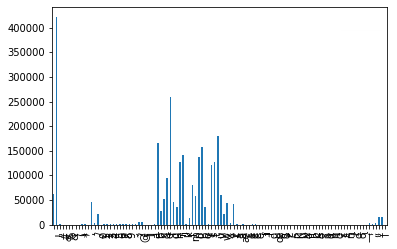
\includegraphics[width=1\textwidth]{images/10_distribution_chars.png} % first figure itself
		\label{fig:distr-chars}
		\caption{All characters}
	\end{minipage}\hfill
	\begin{minipage}{0.5\textwidth}
		\centering
		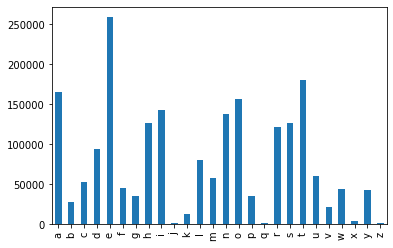
\includegraphics[width=1\textwidth]{images/11_distribution_letters.png} % second figure itself
		\label{fig:distr-letters}
		\caption{Letters (a-z) only}
	\end{minipage}
	\caption{Characters distribution in The Count of Montecristo}
\end{figure}

For completeness, also the top 20 most common characters are shown in table \ref{tab:top-chars}.

\begin{table}[h]
	\caption{Top 20 most common characters in The Count of Montecristo}\label{tab:top-chars}
	\centering
	\begin{tabular}{|l|l|l|}
		\hline
		Position & Character & Frequency \\
		\hline
		\#1 & \textit{space} & 420940 \\
		\#2 & e & 259094 \\
		\#3 & t & 180542 \\
		\#4 & a & 165546 \\
		\#5 & o & 157076 \\
		\#6 & i & 142302 \\
		\#7 & n & 137584 \\
		\#8 & s & 126590 \\
		\#9 & h & 126368 \\
		\#10 & r & 121407 \\
		\#11 & d & 94099 \\
		\#12 & l & 80730 \\
		\#13 & \textit{newline} & 61739 \\
		\#14 & u & 60318 \\
		\#15 & m & 57157 \\
		\#16 & c & 52526 \\
		\#17 & f & 45383 \\
		\#18 & \textit{comma} & 45246 \\
		\#19 & w & 43892 \\
		\#20 & y & 42642 \\
		\#... & ... & ... \\
		\hline
	\end{tabular}
\end{table}

The machine learning dataset has been built by dividing the original text into batches composed by 16 sub-sequences, each 256 characters long. Doing so, a total of 647 batches has been obtained. The training set is composed of all the characters which appear ordered inside the book; the target of each character is the immediately following one, used to actually learning probabilistic sequences generation during the training phase.



\section{Training}

Training has been done using two LSTM cells of 256 units each, through 5 epochs with a learning rate of $10^{-2}$. Figure \ref{fig:loss-total} documents the evolution of the training loss (value on the y-axis) with respect to the epochs (x-axis). Starting from a loss of around 4.67, the fifth epoch reaches a loss that is around 1.30.

In the chart, it can be easily seen that the main improvement is done during the first two epochs, while the next ones are mainly useful for refining the predictions. Figure \ref{fig:loss-epochs} further visualizes this phenomenon: first epoch reaches a loss of about 1.80, improved at 1.50 by the second epoch and decreased to 1.3 during the next three epochs.

\begin{figure}[H]
	\centering
	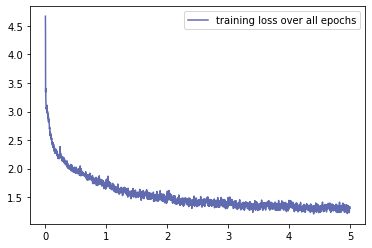
\includegraphics[scale=1]{images/00_loss.png}
	\caption[Training loss over 5 epochs]{Training loss over 5 epochs}
	\label{fig:loss-total}
\end{figure}

\begin{figure}[H]
\centering
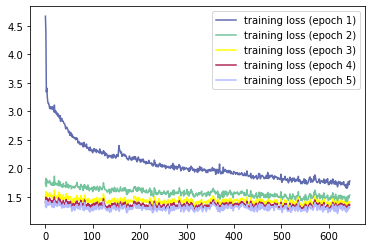
\includegraphics[scale=1]{images/02_loss_all_epochs.png}
\caption[Training loss over 5 epochs]{Training losses for each epoch}
\label{fig:loss-epochs}
\end{figure}




\section{Text generation}

After the training has finished, several sequences (each 256 characters long) have been generated to evaluate the model. The first character has been chosen accordingly to a probability distribution based on the frequency of the characters in the original text.

The result is quite satisfying since, even though the examples have no actual meaning, at least most of the generated tokens are English words. Some examples are reported in the following pages; it can be seen that although without any sense, many of them still have some reasonable structure: take a look at the usage of quotation marks to enclose a direct speech, for example. However, some of the presented generation are really bad.

Please note that few newline characters have been removed for brevity's sake. 
\\

\textbf{Example 1}
\begin{verbatim}
great that i shall propose.
these overed is not astonished your persons with a sive cime,
silence of all paid with astimuts this sleep as this blood, arrived to our
poor fehe. the shade, who tistering to provont
around.”
"what speens with the oldament l
\end{verbatim}

\textbf{Example 2}
\begin{verbatim}
phopped vonie.
"and whom vagered the loably prayers.”
"but do you pleastleds.”
"i understand.”
"alandy was someone,” this croe
as the count and darkness under, whice befalled him, which.
"you received him your mark in his life?”
"that knowsere, 1819,
\end{verbatim}

\textbf{Example 3}
\begin{verbatim}
chuppers of the 
as monte cristo at his letter wills which
last, as it may asked not disposed on molets, wanted this knowledge, 
behind in it, he was cleaned of our fathe

300,000 counten of last surprison in
it. he added any ground. dantès, he opened to wi
\end{verbatim}

\textbf{Example 4}
\begin{verbatim}
ttementor.
"yes,” replied contrardationable.
did you little, sir,” said leanning; "do you promised yourself, then, the
fauther world. there are the wrigue-own—dies,—sine?”
"yes, for you see.”
"how corate, did i do we to receive
them; then, see so herse
\end{verbatim}

\textbf{Example 5}
\begin{verbatim}
 "proprain in de
diese
no one restesing.
speality, but what he knew meeting if she
learning.
he could not kend, marmit and fixed jeine.
"how?”
"yes; distrable understove.” an insufferengness was we peragience. 
andrea observed with a small black.
"pry 
\end{verbatim}

\textbf{Example 6}
\begin{verbatim}
ud her.
"harm!”
"i must will give you the contrary of the sentreage, your wife, as i speak, 
before remained at the little danglars’s stepless you have been acced
for by the same name my hundred tenea, you have here the scene, 
from the garbigul.”
"we shu
\end{verbatim}

\textbf{Example 7}
\begin{verbatim}
ody new deep
assurted by his
face albert,
and enchiverets decondern,
which after walked the carrial
since monte cristo.

"my lord.” cried joined forgottenjes. there were i only
for dantès danglars: and takingly been over, then, in all directions with a con
\end{verbatim}

\textbf{Example 8}
\begin{verbatim}
alland clanted in a fining femous other ala, not knows anyone. do not 
do mellois in possibing arms, and to
know whom you know when when my confidingly name he
pidled me, i come; above the sailed benedetto, i something and
beautifully bright,
and involuting
\end{verbatim}

\textbf{Example 9}
\begin{verbatim}
sf.
"but did not exchana,” said monte cristo. "and where a voice.”
"and then anything carried, nay, monsieur,” said he, in an once 
sacessation informations. and rosped him.

"that keeped
it all thes
promises! is
up with yo
why kind you stared like a
fat
\end{verbatim}

\textbf{Example 10}
\begin{verbatim}
cère who alwars
complipal. professed to
writes filled into.

monte cristo’s gentlemen was away, the door were alone fine door 
addid monte cristo?”

18471  as there. "the light that.”

"well, it is very horse—no was at sight of the lateorice you dies.”
"s
\end{verbatim}

\textbf{Example 11}
\begin{verbatim}
t7; three to the bescuite
carriagezing princess, nearly ventuace
came his brow.

"you are alone—come.”
"well.”
"yes,” said he tode valunive
steward to use and madness either and father conversing the fixe them,
but to took that.

beings revengered, seeme
\end{verbatim}

\textbf{Example 12}
\begin{verbatim}
ex, he a side, and whi
had gived him fernand.

"i do not.”
"gentlemen, for his three door would not like any werr equal young.” 
they knews and smokes.

40168m

"yes,” said the worthence which awger, the light, and poterewself him to the
new order. never
\end{verbatim}

\textbf{Example 13}
\begin{verbatim}
refully, "no one she flone, which, door alone like a so
good accuranger prifalry at laboage.”

"at the despercuis
for
procopy?—i magrandely, to ever experis; his isservants, 
they must be well efforts.”

30019m
"and twering three the teneht, and it, i ha
\end{verbatim}

\textbf{Example 14}
\begin{verbatim}
nanded with villefort’s light to this wedtings, and sparkless serv 
this head of seeing.

"but i not?”

"now,” said monte’s streeek), and of the indering well-beated declections 
into t enfort of monte ceip, and whom m. 29 temptened evereted from blispold ex
\end{verbatim}

\textbf{Example 15}
\begin{verbatim}
—”

"yes,” said bentive increasing, stood innocribited naysuilh; 
expressed being right, and dargeely its
riches
toscees
in his enemy. at, but th t
expleaus
gutful
and inform the
steps where
for an hour of his father that everything was
not alarmed
them a p
\end{verbatim}

\textbf{Example 16}
\begin{verbatim}
asturmed, ah, dressen. shat sunled whether the
particulars. the acquaintess with their girl. then, on as demands thrrught of the
exclay of things which

every
door, learnes, and that comrades ece—willing
mad,
never overcapted morcerf on his sor so eyes tha
\end{verbatim}

\textbf{Example 17}
\begin{verbatim}
im of the frwit one as bursost bluppomor, so with

information shall then spertic and
curious ritading that a privaxe a count’s descarcely ginding mith these occhinated
swen
for severates to still
alid who
then returned to began to
liberables with extrah, 
\end{verbatim}

\textbf{Example 18}
\begin{verbatim}
sthosed on the particant confine, it is see into the very gardenum 
forgeaveling chaborts of the
senstions which nervess
had even strawseres on the same approod from times.

morrel with asseding a whore to
unarkilated to become that he is that she looked an
\end{verbatim}

\textbf{Example 19}
\begin{verbatim}
ngial
to a sign.

under nor. in a shadow
and public, which descended to the opera much; and he project gut
opens wherespealed
crounced by the
moment,
for as a hundred by a chibino
documents of occupied upains. not
the house, becomes t
came; through an
air,
\end{verbatim}

\textbf{Example 20}
\begin{verbatim}
l
has deficied the storm, stronged to ask it with a side-podery l
off it, it is franz. 
706112
031(m
sutmos caat,” said
ever from,”
replied dantès, and
trauspiences, little veloneess get one to his hearth;
"but by the usual of the islemen, old expect
\end{verbatim}




%\section{Model Improvement}







\end{document}